\begin{highlightblock}[Delta ADC (Nachlaufumsetzer)]

\begin{center}
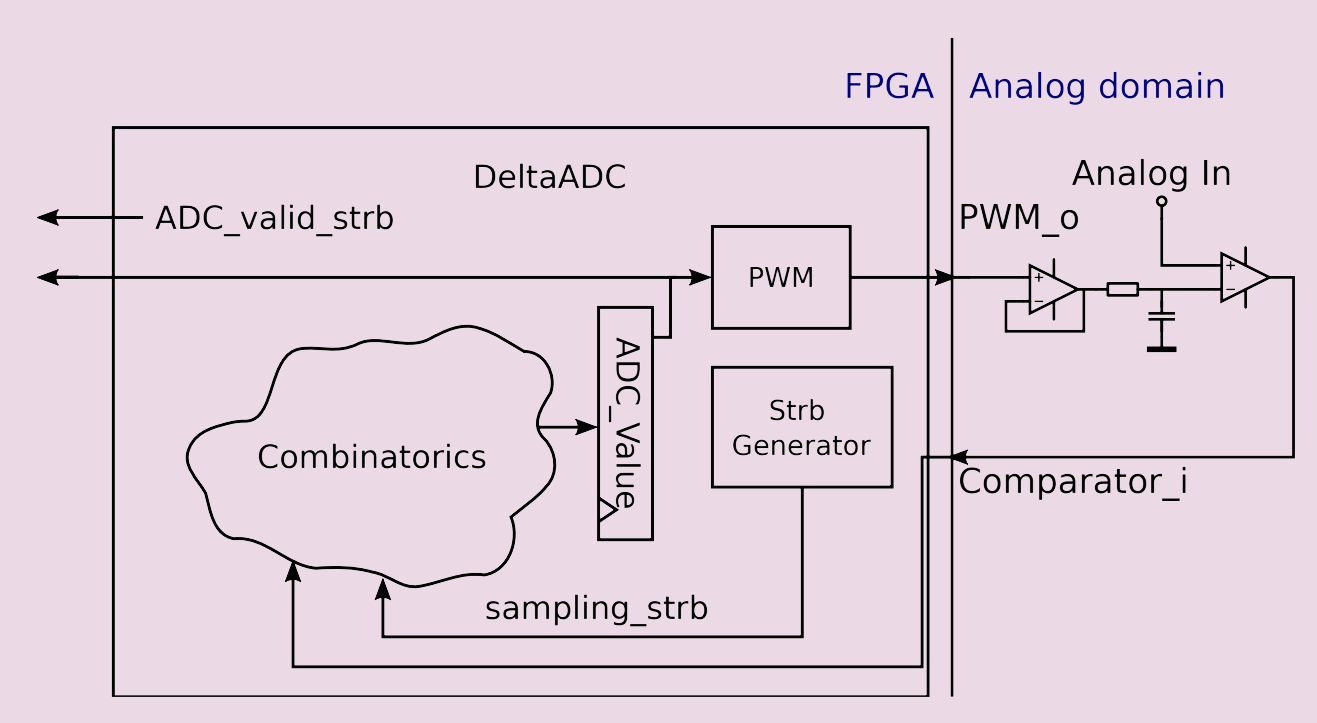
\includegraphics[width=0.7\linewidth]{images/DeltaADC-Block.png}

Figure \refstepcounter{figure}\arabic{figure}: Delta ADC Block\label{fig:delta_adc}
\end{center}

In this exercise, we will start the digital design of a delta ADC, schematically
shown in Figure \ref{fig:delta_adc}. It works like the following. A PWM Signal generated by the
FPGA is output through an analog low pass filter (more details on the analog
part will follow in a future exercise), resulting in a voltage level that is compared
to the analog input via an analog comparator. This comparator outputs a zero if
the analog input is lower than the comparison voltage level and a one otherwise.
In the digital domain the comparator signal (Comparator i) is used to increase
the ADC value in case Comparator i is one and decrease the ADC value in case
Comparator i is zero. A change of the ADC value should only occur at rising
clock edges where the sampling strobe (sampling strb) generated by a strobe
generator is one. This will lead to a sampling that is equidistantly spaced in
time with the sampling frequency defined by the frequency of sampling strb.
The ADC value is feed to the PWM to define the ON counter val i. This way a
simple control loop is closed, allowing the ADC value to adapt to analog signal.
This way the ADC signal will follow the analog signal with its value proportional
(up to an adjustment error) to the analog input.
\end{highlightblock}

\begin{highlightblock}[To-Do-List]
\begin{itemize}
    \item Draw a block diagram of the required combinatorics. Do you need to
        have
a finite state machine? If you do, please write a state diagram.
    \item Draw the required blocks to the block diagram for implementing the
        signal ADC valid strb.
    \item Write the entities and architectures that are required in VHDL. As
        you did not design the strobe generator yet it is suggested that you
        start with the strobe generator. Find meaningful generics such that the
        frequency of the strobe generator is adjustable (you might set the time
        between strobes to a few clock cycles for the simulation, however for
        future use several thousands of clock cycles might be required). Use
        one .vhd file for each entity and one .vhd file for each architecture.
    \item Write a testbench in VHDL (extra file). Simulate the system using
        Modelsim and hand in screenshots showing the output of the waveform
        window. Find meaningful test cases. As you are not able to simulate the
        analog domain, your testbench can only simulate the behavior of the
        comparator input. What are meaningful testcases for Comparator i to
        adequately simulate the designs behavior.
    \item Discuss the results of the simulation in a few sentences and answer
        the questions.
\end{itemize}
\end{highlightblock}
